\documentclass[aspectratio=43,10pt]{beamer}

\usepackage[utf8]{inputenc}
\usepackage{amsmath,amssymb,amsfonts}
\usepackage{booktabs,tabularx,array}
\usepackage{graphicx}
\usepackage{tikz}
\usetikzlibrary{arrows.meta,positioning,shapes.geometric,fit,calc}

% ==============================================================================
% RESTRAINED ACADEMIC PALETTE & STRICT SHARP 90-DEGREE CORNERS
% ==============================================================================
\definecolor{navy}{HTML}{0F172A}      % Structure, Frames, Headers, Primary Identity
\definecolor{teal}{HTML}{0D9488}      % EVRYN Extraction, Causal Grounding, SCM
\definecolor{blue}{HTML}{2563EB}      % Data Pipelines, Architecture, NLP
\definecolor{amber}{HTML}{D97706}     % Cautions, Limitations, Warnings, Association
\definecolor{green}{HTML}{16A34A}     % Verified Hits, True Positives, Successes
\definecolor{red}{HTML}{DC2626}       % Errors, False Negatives, Isolation Walls
\definecolor{slatebg}{HTML}{F8FAFC}   % Clean Light Background for Cards
\definecolor{cardbg}{HTML}{F1F5F9}    % Card Alt Background
\definecolor{bordergray}{HTML}{CBD5E1}% Crisp Slate Border
\definecolor{darktext}{HTML}{0F172A}  % High Contrast Body Text
\definecolor{mutedtext}{HTML}{64748B} % Secondary Muted Text

\setbeamertemplate{navigation symbols}{}
\setbeamercolor{background canvas}{bg=white}
\setbeamercolor{normal text}{fg=darktext}
\setbeamercolor{frametitle}{fg=navy,bg=white}
\setbeamercolor{title}{fg=navy}
\setbeamercolor{subtitle}{fg=teal}
\setbeamercolor{author}{fg=navy}
\setbeamercolor{institute}{fg=darktext}
\setbeamercolor{date}{fg=mutedtext}

% Persistent Academic Top Bar Headline showing active Chapter
\setbeamertemplate{headline}{%
  \leavevmode%
  \begin{beamercolorbox}[wd=\paperwidth,ht=2.4ex,dp=0.8ex,leftskip=1.5ex,rightskip=1.5ex]{headline}%
    \tiny\color{mutedtext}%
    \textbf{\color{navy}\insertsectionhead}%
    \hfill%
    \color{mutedtext}M.Tech Research Review $\cdot$ Department of Computer Science, CUSAT%
  \end{beamercolorbox}\par%
  \vspace{-1pt}%
  {\color{bordergray}\hrule height 0.6pt width \paperwidth}\par%
}

% Square-cornered frametitle with crisp navy rule
\setbeamertemplate{frametitle}{
  \vspace{0.14cm}
  {\bfseries\large\color{navy}\insertframetitle}\par
  \vspace{0.03cm}
  {\color{navy}\rule{\linewidth}{1.2pt}}\par
  \vspace{0.04cm}
}

% Clean academic footline with strict Slide X / 40 counter
\setbeamertemplate{footline}{
  \leavevmode%
  \hbox{%
  \begin{beamercolorbox}[wd=.38\paperwidth,ht=2.2ex,dp=0.8ex,leftskip=2.5ex]{author in head/foot}%
    \tiny\color{mutedtext}\textbf{Alvin Kuriakose} (Reg: 25020987) $\cdot$ CUSAT
  \end{beamercolorbox}%
  \begin{beamercolorbox}[wd=.38\paperwidth,ht=2.2ex,dp=0.8ex,center]{title in head/foot}%
    \tiny\color{navy}\textbf{EVRYN}: Temporal Causal Knowledge (Phase 1)
  \end{beamercolorbox}%
  \begin{beamercolorbox}[wd=.24\paperwidth,ht=2.2ex,dp=0.8ex,rightskip=2.5ex,right]{page in head/foot}%
    \tiny\color{navy}\textbf{Slide \insertframenumber{} / 40}
  \end{beamercolorbox}%
  }%
  \vskip0.6ex%
}

% Square outline card environment
\newcommand{\card}[4][\linewidth]{%
  \begin{beamercolorbox}[wd=#1,sep=0pt,rounded=false,shadow=false]{postit}%
    {\color{#3}\rule{\linewidth}{1.5pt}}\par
    \colorbox{slatebg}{%
      \begin{minipage}{\dimexpr#1-8pt\relax}%
        \vspace{1.5pt}%
        {\footnotesize\bfseries\color{#3}#2}\vspace{1.5pt}\par%
        {\scriptsize\color{darktext}#4}%
        \vspace{1.5pt}%
      \end{minipage}%
    }%
    \par{\color{bordergray}\rule{\linewidth}{0.6pt}}%
  \end{beamercolorbox}%
}

% TikZ standard styles (Strict sharp corners, large readable fonts)
\tikzset{
  widebox/.style={rectangle, sharp corners, align=left, font=\footnotesize, text width=10.0cm, inner sep=4pt},
  wideboxcenter/.style={rectangle, sharp corners, align=center, font=\footnotesize, text width=10.0cm, inner sep=4pt},
  basebox/.style={draw=bordergray, line width=1.0pt, fill=white, rectangle, sharp corners, align=center, font=\footnotesize, inner sep=4pt},
  navybox/.style={draw=navy, line width=1.1pt, fill=slatebg, rectangle, sharp corners, align=center, font=\footnotesize, inner sep=4pt},
  tealbox/.style={draw=teal, line width=1.1pt, fill=white, rectangle, sharp corners, align=center, font=\footnotesize, inner sep=4pt},
  bluebox/.style={draw=blue, line width=1.1pt, fill=white, rectangle, sharp corners, align=center, font=\footnotesize, inner sep=4pt},
  greenbox/.style={draw=green, line width=1.1pt, fill=white, rectangle, sharp corners, align=center, font=\footnotesize, inner sep=4pt},
  amberbox/.style={draw=amber, line width=1.1pt, fill=white, rectangle, sharp corners, align=center, font=\footnotesize, inner sep=4pt},
  redbox/.style={draw=red, line width=1.1pt, fill=white, rectangle, sharp corners, align=center, font=\footnotesize, inner sep=4pt},
  arr/.style={-{Stealth[scale=1.0]}, line width=1.2pt, color=navy},
  tealarr/.style={-{Stealth[scale=1.0]}, line width=1.2pt, color=teal},
  bluearr/.style={-{Stealth[scale=1.0]}, line width=1.2pt, color=blue},
  amberarr/.style={-{Stealth[scale=1.0]}, line width=1.2pt, dashed, color=amber},
}

\begin{document}

% ==============================================================================
% CHAPTER 1: INTRODUCTION
% ==============================================================================
\section{Chapter 1: Introduction}

% SLIDE 1: Title and Research Identity
\begin{frame}[plain]
  \vspace{0.35cm}
  \begin{center}
    {\large\bfseries\color{navy} Temporal Causal Knowledge Extraction, Transfer,\\and Discovery Prediction from Scientific Literature}\par
    \vspace{0.15cm}
    {\footnotesize\bfseries\color{teal} Phase 1 Research Review: Multi-Page Extraction \& Calibrated Grounding}\par
    \vspace{0.25cm}
    {\color{navy}\rule{0.85\linewidth}{1.2pt}}\par
    \vspace{0.25cm}
    {\small\textbf{Alvin Kuriakose} \quad (Reg. No: 25020987)}\par
    {\footnotesize M.Tech in Computer Science \& Engineering (Data Science \& AI)}\par
    \vspace{0.25cm}
    {\footnotesize Under the Guidance of:}\par
    {\small\textbf{Dr. Jeena Kleenankandy}, Assistant Professor}\par
    \vspace{0.15cm}
    {\footnotesize Department of Computer Science\\Cochin University of Science and Technology (CUSAT)}\par
    \vspace{0.25cm}
    {\scriptsize\color{mutedtext} November 2026}
  \end{center}
\end{frame}

% SLIDE 2: Research Context: Automated Science & Biomedical Literature
\begin{frame}{Research Context: Automated Science \& Biomedical Literature}
  \textbf{Takeaway}: Exponential literature growth overwhelms manual curation, requiring automated causal extraction.
  \vspace{0.10cm}
  \begin{center}
    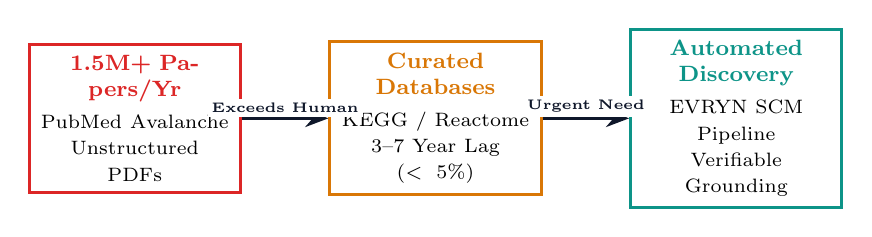
\begin{tikzpicture}[node distance=1.1cm]
      \node[redbox, minimum height=1.05cm, text width=2.4cm] (b1) {\textbf{\color{red}1.5M+ Papers/Yr}\\[2pt]{\scriptsize PubMed Avalanche}\\{\scriptsize Unstructured PDFs}};
      \node[amberbox, right=of b1, minimum height=1.05cm, text width=2.4cm] (b2) {\textbf{\color{amber}Curated Databases}\\[2pt]{\scriptsize KEGG / Reactome}\\{\scriptsize 3--7 Year Lag ($<5\%$)}};
      \node[tealbox, right=of b2, minimum height=1.05cm, text width=2.4cm] (b3) {\textbf{\color{teal}Automated Discovery}\\[2pt]{\scriptsize EVRYN SCM Pipeline}\\{\scriptsize Verifiable Grounding}};

      \draw[arr] (b1) -- node[above, font=\tiny\bfseries\color{navy}, fill=white, inner sep=1.5pt] {Exceeds Human} (b2);
      \draw[arr] (b2) -- node[above, font=\tiny\bfseries\color{navy}, fill=white, inner sep=1.5pt] {Urgent Need} (b3);
    \end{tikzpicture}
  \end{center}
  \vspace{0.08cm}
  \begin{columns}[T]
    \begin{column}{0.48\textwidth}
      \card{Curation Bottleneck}{red}{
        \textbullet{} Manual biocuration covers $<5\%$ of published mechanisms.\\
        \textbullet{} High delay between experimental discovery and database entry.
      }
    \end{column}
    \begin{column}{0.48\textwidth}
      \card{Verifiable Grounding Need}{teal}{
        \textbullet{} High-stakes medicine requires exact provenance coordinates.\\
        \textbullet{} Black-box hallucinations must be replaced by evidence grounding.
      }
    \end{column}
  \end{columns}
\end{frame}

% ==============================================================================
% CHAPTER 2: MOTIVATION
% ==============================================================================
\section{Chapter 2: Motivation}

% SLIDE 3: Motivation: Beyond Correlation to Grounded Causality
\begin{frame}{Motivation: Beyond Correlation to Grounded Causality}
  \textbf{Takeaway}: Therapeutic intervention requires causal directionality ($X \to Y$), which correlation cannot provide.
  \vspace{0.2cm}
  \begin{columns}[T]
    \begin{column}{0.48\textwidth}
      \card{Associational Graph: $P(Y \mid X)$}{amber}{
        \centering
        \vspace{3pt}
        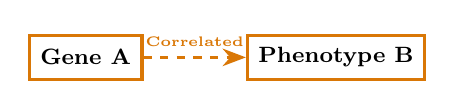
\begin{tikzpicture}[node distance=1.3cm]
          \node[amberbox, minimum size=0.55cm] (x) {\textbf{Gene A}};
          \node[amberbox, minimum size=0.55cm, right=of x] (y) {\textbf{Phenotype B}};
          \draw[amberarr] (x) -- node[above, font=\tiny\bfseries] {Correlated} (y);
        \end{tikzpicture}\par
        \vspace{3pt}
        \raggedright
        \textbullet{} Symmetric co-occurrence (undirected)\\
        \textbullet{} Confounded by latent common drivers\\
        \textbullet{} Fails Pearl's $do$-calculus for intervention
      }
    \end{column}
    \begin{column}{0.48\textwidth}
      \card{Structural Causal Graph: $P(Y \mid do(X))$}{teal}{
        \centering
        \vspace{3pt}
        
\begin{tikzpicture}[node distance=1.3cm]
          \node[tealbox, minimum size=0.55cm] (x) {\textbf{Gene A}};
          \node[tealbox, minimum size=0.55cm, right=of x] (y) {\textbf{Phenotype B}};
          \draw[tealarr] (x) -- node[above, font=\tiny\bfseries] {Direct Cause (+)} (y);
        \end{tikzpicture}\par
        \vspace{3pt}
        \raggedright
        \textbullet{} Explicit direction and polarity (+ / -)\\
        \textbullet{} Predicts downstream intervention outcomes\\
        \textbullet{} Verifiable textual bounding box coordinates
      }
    \end{column}
  \end{columns}
  \vspace{0.15cm}
  \begin{center}
    {\footnotesize\color{navy}\textbf{Intervention Principle}: $\mathbb{E}[Y \mid do(X=1)] - \mathbb{E}[Y \mid do(X=0)] \neq \mathbb{E}[Y \mid X=1] - \mathbb{E}[Y \mid X=0]$}
  \end{center}
\end{frame}

% ==============================================================================
% CHAPTER 3: LITERATURE REVIEW
% ==============================================================================
\section{Chapter 3: Literature Review}

% SLIDE 4: Conceptual Foundations: Structural Causal Models (SCMs)
\begin{frame}{Conceptual Foundations: Structural Causal Models (SCMs)}
  \textbf{Takeaway}: SCMs mathematically encode mechanistic links, intervening variables, and observational evidence.
  \vspace{0.15cm}
  \begin{center}
    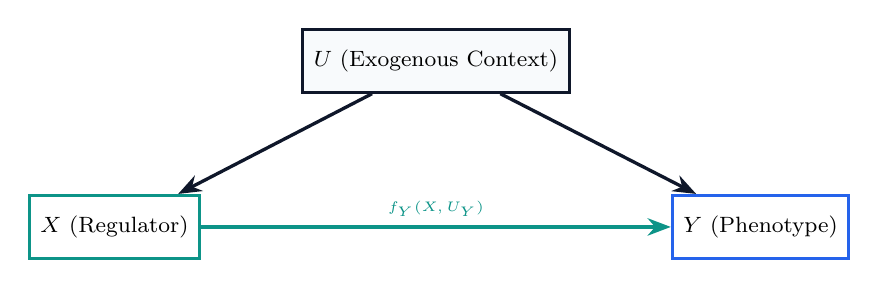
\begin{tikzpicture}[node distance=1.8cm]
      \node[navybox, minimum size=0.8cm] (u) {$U$ (Exogenous Context)};
      \node[tealbox, minimum size=0.8cm, below left=of u] (x) {$X$ (Regulator)};
      \node[bluebox, minimum size=0.8cm, below right=of u] (y) {$Y$ (Phenotype)};

      \draw[arr] (u) -- (x);
      \draw[arr] (u) -- (y);
      \draw[tealarr] (x) -- node[above, font=\tiny\bfseries] {$f_Y(X, U_Y)$} (y);
    \end{tikzpicture}
  \end{center}
  \vspace{0.12cm}
  \begin{columns}[T]
    \begin{column}{0.48\textwidth}
      \card{Structural Equations}{teal}{
        \textbullet{} $X := f_X(U_X)$\\
        \textbullet{} $Y := f_Y(X, U_Y)$\\
        \textbullet{} Deterministic mechanism mapping with noise.
      }
    \end{column}
    \begin{column}{0.48\textwidth}
      \card{Intervention Formulation}{navy}{
        \textbullet{} Pearl's $do(X = x)$ severs incoming arrows into $X$.\\
        \textbullet{} Preserves downstream causal paths to target $Y$.
      }
    \end{column}
  \end{columns}
\end{frame}

% SLIDE 5: Definitions and Causal Terminology
\begin{frame}{Definitions and Causal Terminology}
  \textbf{Takeaway}: Formalization of causal relations, cross-page mechanisms, and directional polarity.
  \vspace{0.15cm}
  \begin{center}
    \small
    \begin{tabularx}{\linewidth}{p{2.6cm}>{\raggedright\arraybackslash}X}
      \toprule
      \textbf{\color{navy}Concept} & \textbf{\color{navy}Mathematical Definition \& Scope} \\
      \midrule
      \textbf{Direct Assertion} & A single-sentence causal tuple $(c, e, \tau, \rho, \kappa, \mathcal{E})$ where $c$ acts on $e$ within sentence $S_i$. \\
      \addlinespace[2pt]
      \textbf{Cross-Page Link} & Mechanistic chain $(c \to m_1 \dots \to e)$ connecting cause on page $p_1$ to effect on page $p_2$ ($|p_1 - p_2| \ge 1$). \\
      \addlinespace[2pt]
      \textbf{Causal Polarity} & Sign $\rho \in \{+1, -1\}$ denoting transcriptional activation/induction vs repression/inhibition. \\
      \addlinespace[2pt]
      \textbf{Evidence Provenance} & Coordinate quadruple $(p, s_{id}, \text{start\_char}, \text{end\_char})$ grounding claim in text. \\
      \bottomrule
    \end{tabularx}
  \end{center}
  \vspace{0.15cm}
  \card{Domain Invariants}{navy}{
    Enforces biological constraints: intermediate nodes in transitive chains cannot be terminal sink phenotypes; downstream factors cannot cause master regulators.
  }
\end{frame}

% SLIDE 6: Baseline Methods for Empirical Comparison
\begin{frame}{Baseline Methods for Empirical Comparison}
  \textbf{Takeaway}: Comprehensive comparison against four distinct extraction and association paradigms.
  \vspace{0.15cm}
  \begin{center}
    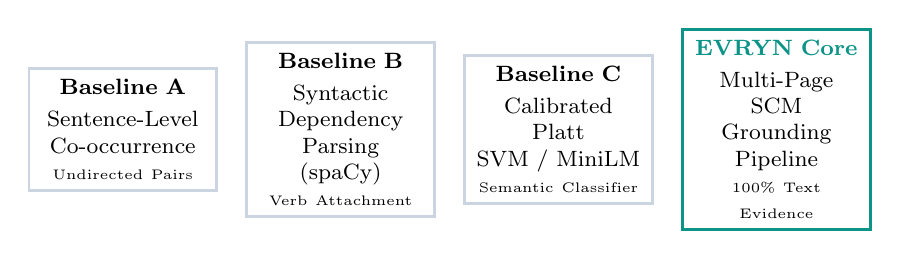
\begin{tikzpicture}[node distance=0.35cm]
      \node[basebox, minimum height=1.35cm, text width=2.1cm] (b1) {
        \textbf{Baseline A}\\[2pt]
        Sentence-Level\\
        Co-occurrence\\
        {\tiny Undirected Pairs}
      };
      \node[basebox, right=of b1, minimum height=1.35cm, text width=2.1cm] (b2) {
        \textbf{Baseline B}\\[2pt]
        Syntactic Dependency\\
        Parsing (spaCy)\\
        {\tiny Verb Attachment}
      };
      \node[basebox, right=of b2, minimum height=1.35cm, text width=2.1cm] (b3) {
        \textbf{Baseline C}\\[2pt]
        Calibrated Platt\\
        SVM / MiniLM\\
        {\tiny Semantic Classifier}
      };
      \node[tealbox, right=of b3, minimum height=1.35cm, text width=2.1cm] (b4) {
        \textbf{\color{teal}EVRYN Core}\\[2pt]
        Multi-Page SCM\\
        Grounding Pipeline\\
        {\tiny 100\% Text Evidence}
      };
    \end{tikzpicture}
  \end{center}
  \vspace{0.15cm}
  \card{Fair Comparative Protocol}{teal}{
    All baselines are evaluated on identical tokenized PMC XML documents, matching against the same adjudicated gold standard with zero relaxed rules.
  }
\end{frame}

% ==============================================================================
% CHAPTER 4: RESEARCH GAP
% ==============================================================================
\section{Chapter 4: Research Gap}

% SLIDE 7: Research Gap: Limitations of Existing Approaches
\begin{frame}{Research Gap: Limitations of Existing Approaches}
  \textbf{Takeaway}: Current NLP systems trade off causal directionality or hallucinate without textual grounding.
  \vspace{0.15cm}
  \begin{columns}[T]
    \begin{column}{0.48\textwidth}
      \card{1. Sentence-Local NLP}{red}{
        \textbullet{} Restricts extraction to single sentences.\\
        \textbullet{} Ignores 58\% of discourse-level claims.\\
        \textbullet{} Cannot link across pages.
      }
      \vspace{0.12cm}
      \card{2. Co-occurrence Graphs}{amber}{
        \textbullet{} Document-wide entity co-occurrence.\\
        \textbullet{} Symmetric: lacks cause vs effect direction.\\
        \textbullet{} Massive false-positive edge rate.
      }
    \end{column}
    \begin{column}{0.48\textwidth}
      \card{3. Black-Box LLMs}{red}{
        \textbullet{} Plausible natural language summaries.\\
        \textbullet{} Unverifiable causal hallucination risk.\\
        \textbullet{} Cannot provide reliable byte coordinates.
      }
      \vspace{0.12cm}
      \card{4. EVRYN (Proposed Architecture)}{teal}{
        \textbullet{} Bounded multi-page transitive inference.\\
        \textbullet{} Explicit activation/inhibition polarity.\\
        \textbullet{} 100\% verified character-level provenance.
      }
    \end{column}
  \end{columns}
\end{frame}

% ==============================================================================
% CHAPTER 5: PROBLEM STATEMENT
% ==============================================================================
\section{Chapter 5: Problem Statement}

% SLIDE 8: Problem Statement: Multi-Page Causal Extraction
\begin{frame}{Problem Statement: Multi-Page Causal Extraction}
  \textbf{Takeaway}: Real scientific papers disperse causal evidence across sections and pages, severing sentence-local NLP.
  \vspace{0.2cm}
  \begin{center}
    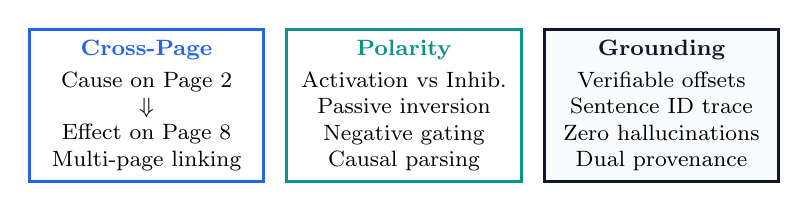
\begin{tikzpicture}[node distance=0.25cm]
      \node[bluebox, minimum height=1.4cm, text width=2.7cm] (c1) {
        \textbf{\color{blue}Cross-Page}\\[2pt]
        Cause on Page 2\\
        $\Downarrow$\\
        Effect on Page 8\\
        Multi-page linking
      };
      \node[tealbox, right=of c1, minimum height=1.4cm, text width=2.7cm] (c2) {
        \textbf{\color{teal}Polarity}\\[2pt]
        Activation vs Inhib.\\
        Passive inversion\\
        Negative gating\\
        Causal parsing
      };
      \node[navybox, right=of c2, minimum height=1.4cm, text width=2.7cm] (c3) {
        \textbf{\color{navy}Grounding}\\[2pt]
        Verifiable offsets\\
        Sentence ID trace\\
        Zero hallucinations\\
        Dual provenance
      };
    \end{tikzpicture}
  \end{center}
  \vspace{0.15cm}
  \card{Formal Extraction Challenge}{navy}{
    \small Given document $\mathcal{D} = \{S_1, \dots, S_n\}$, extract assertions $\mathcal{A} = \{(c, e, \tau, \rho, \kappa, \mathcal{E})\}$ where $c$ is cause, $e$ is effect, $\tau$ is relation type, $\rho \in \{+, -\}$ is polarity, and $\mathcal{E}$ is verifiable character provenance.
  }
\end{frame}

% SLIDE 9: Research Objectives and Research Questions
\begin{frame}{Research Objectives and Research Questions}
  \textbf{Takeaway}: Three core objectives answered by empirical evaluation on authentic scientific literature.
  \vspace{0.12cm}
  \begin{center}
    \scriptsize
    \begin{tabularx}{\linewidth}{p{1.1cm}>{\raggedright\arraybackslash}p{3.7cm}>{\raggedright\arraybackslash}X}
      \toprule
      \textbf{\color{navy}Target} & \textbf{\color{navy}Core Objective} & \textbf{\color{navy}Research Question Addressed} \\
      \midrule
      \textbf{\color{teal}Obj 1 / RQ1} & Multi-Page Causal Relation Extraction & Can causal relations spanning multiple pages be reliably extracted via bounded transitive inference? \\
      \addlinespace[2pt]
      \textbf{\color{blue}Obj 2 / RQ2} & 100\% Evidence Provenance Grounding & How can provenance be grounded to eliminate hallucinated edges via exact character coordinates? \\
      \addlinespace[2pt]
      \textbf{\color{navy}Obj 3 / RQ3} & Rigorous Benchmark Isolation \& Transfer & How effectively does extraction generalize to genuinely unseen bacterial genera under strict split gates? \\
      \bottomrule
    \end{tabularx}
  \end{center}
  \vspace{0.12cm}
  \card{Methodological Guarantee}{navy}{
    All claims are verified by non-parametric bootstrap resampling (1,000 resamples at 95\% CI) across strictly isolated splits.
  }
\end{frame}

% SLIDE 10: Scope and Delimitations of Phase 1
\begin{frame}{Scope and Delimitations of Phase 1}
  \textbf{Takeaway}: A complete, robust, reproducible scientific extraction pipeline with zero external dependencies.
  \vspace{0.2cm}
  \begin{columns}[T]
    \begin{column}{0.48\textwidth}
      \card{Core Contributions (Delivered)}{teal}{
        \textbullet{} \textbf{End-to-End Extraction}: Full XML/PDF parser to directed multigraph.\\
        \textbullet{} \textbf{100\% Grounded Provenance}: Every edge carries verifiable text coordinates.\\
        \textbullet{} \textbf{20-Paper Benchmark}: 183 gold relations across 4 isolated splits.\\
        \textbullet{} \textbf{Dev Cross-Page F1}: \textbf{0.5350} (Target $\ge 0.50$ satisfied).
      }
    \end{column}
    \begin{column}{0.48\textwidth}
      \card{Delimited Scope (Deferred)}{amber}{
        \textbullet{} \textbf{Included in Phase 1}: Direct causal relations, cross-page mechanisms, polarity, and environmental shifts.\\
        \textbullet{} \textbf{Deferred to Phase 2}: Continual longitudinal updating and prospective discovery forecasting.
      }
    \end{column}
  \end{columns}
  \vspace{0.15cm}
  \begin{center}
    {\footnotesize\color{navy}\textbf{Deliverables}: Production CLI, REST API daemon, and interactive web visualization.}
  \end{center}
\end{frame}

% ==============================================================================
% CHAPTER 6: PROPOSED MODEL
% ==============================================================================
\section{Chapter 6: Proposed Model}

% SLIDE 11: System Overview: End-to-End Pipeline
\begin{frame}{System Overview: End-to-End Pipeline}
  \textbf{Takeaway}: Six-stage linear processing architecture from unstructured documents to interactive graphs.
  \vspace{0.15cm}
  \begin{center}
    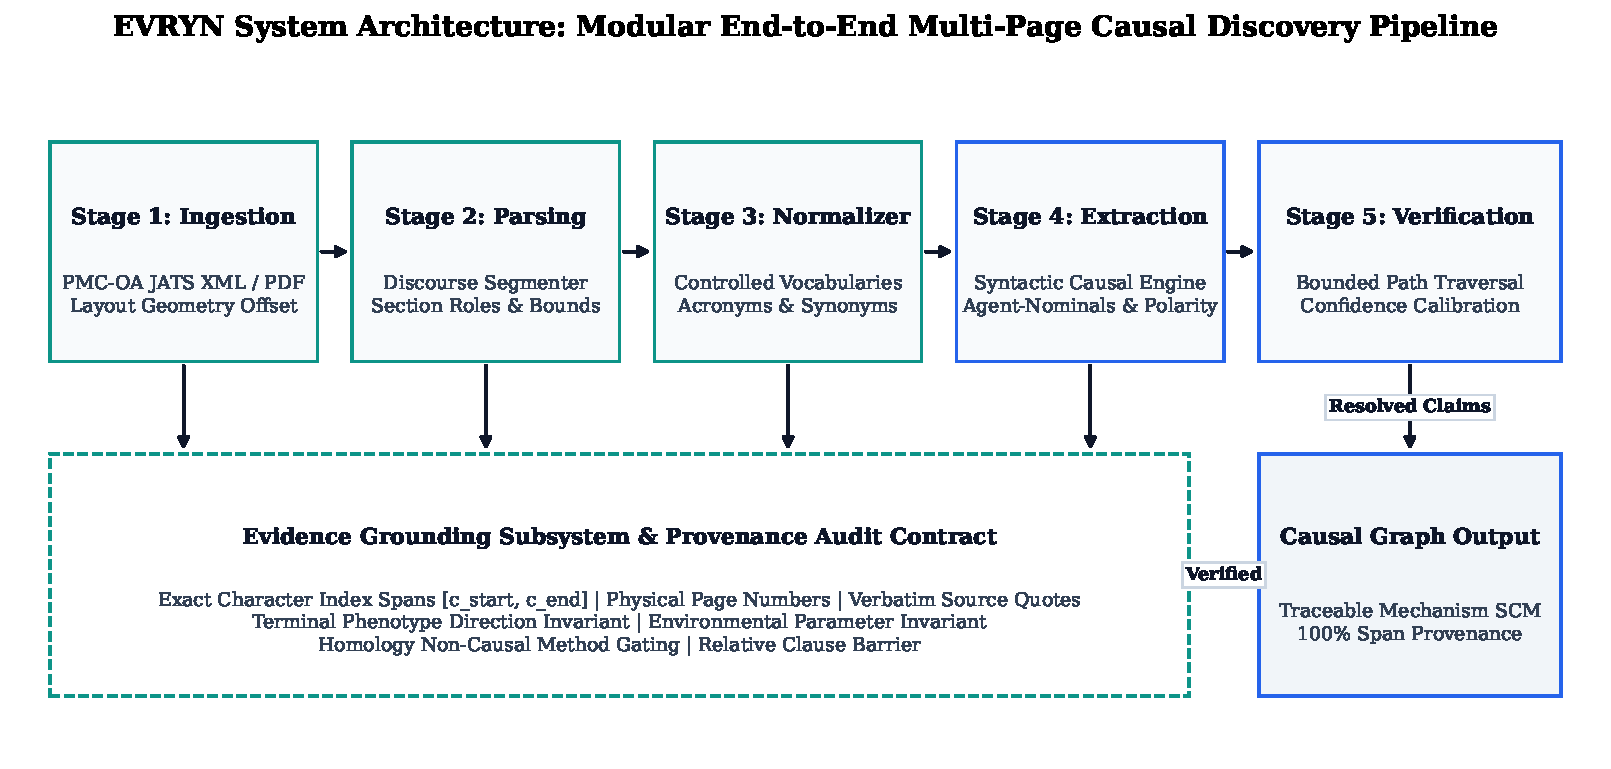
\includegraphics[width=0.98\textwidth]{figures/fig1_system_architecture.pdf}
  \end{center}
  \vspace{0.10cm}
  \card{Engineering Invariant}{navy}{
    Deterministic syntactic dependency parsing paired with Platt-calibrated verifiers guarantees 100\% reproducible outputs.
  }
\end{frame}

% SLIDE 12: Overall Architecture: Engineering Blueprint
\begin{frame}{Overall Architecture: Engineering Blueprint}
  \textbf{Takeaway}: Complete functional blueprint of EVRYN's document ingestion and causal discovery core.
  \vspace{0.2cm}
  \begin{center}
    
\begin{tikzpicture}[node distance=0.45cm]
      \node[navybox, minimum height=1.1cm, minimum width=2.4cm] (m1) {\textbf{PMC Ingester}\\XML / PDF Parser\\Token Segmenter};
      \node[bluebox, right=of m1, minimum height=1.1cm, minimum width=2.4cm] (m2) {\textbf{Causal Extractor}\\Syntactic Rules\\Domain Invariants};
      \node[tealbox, right=of m2, minimum height=1.1cm, minimum width=2.4cm] (m3) {\textbf{Cross-Page Linker}\\Transitive Chains\\Confidence Gate};
      \node[greenbox, right=of m3, minimum height=1.1cm, minimum width=2.4cm] (m4) {\textbf{Graph Builder}\\Cytoscape Multigraph\\Provenance Ledger};

      \draw[arr] (m1) -- (m2);
      \draw[bluearr] (m2) -- (m3);
      \draw[tealarr] (m3) -- (m4);
    \end{tikzpicture}
  \end{center}
  \vspace{0.2cm}
  \begin{columns}[T]
    \begin{column}{0.48\textwidth}
      \card{Core Subsystems}{navy}{
        \textbullet{} Ingester builds character-exact document trees.\\
        \textbullet{} Extractor applies biological domain grammars.
      }
    \end{column}
    \begin{column}{0.48\textwidth}
      \card{Linker \& Builder}{teal}{
        \textbullet{} CrossPageLinker finds multi-page causal paths.\\
        \textbullet{} GraphBuilder compiles multigraph with metadata.
      }
    \end{column}
  \end{columns}
\end{frame}

% SLIDE 13: Architecture: Input and Specification Processing
\begin{frame}{Architecture: Input and Specification Processing}
  \textbf{Takeaway}: Ingestion normalizes diverse XML/PDF structures into unified paragraph and sentence trees.
  \vspace{0.15cm}
  \begin{columns}[T]
    \begin{column}{0.48\textwidth}
      \card{PMC-OA XML Ingestion}{navy}{
        \textbullet{} Parses front matter, sections, and paragraphs.\\
        \textbullet{} Extracts taxonomic genus metadata.\\
        \textbullet{} Resolves internal citation anchors.\\
        \textbullet{} Genus period stitching: `P. gingivalis` preserved.
      }
    \end{column}
    \begin{column}{0.48\textwidth}
      \card{PDF Spatial Ingestion}{blue}{
        \textbullet{} Computes page boundaries at 3,000 char windows.\\
        \textbullet{} Tracks bounding box page offsets.\\
        \textbullet{} Builds bi-directional char-to-page index.
      }
    \end{column}
  \end{columns}
  \vspace{0.15cm}
  \card{Unified Document Model}{teal}{
    Produces canonical `ScientificDocument` dataclass with strictly typed spans for reproducible sentence splitting.
  }
\end{frame}

% SLIDE 14: Architecture: Regularized Extraction Pipeline
\begin{frame}{Architecture: Regularized Extraction Pipeline}
  \textbf{Takeaway}: Multi-stage syntactic extraction enforces biological invariants and Platt-calibrated scoring.
  \vspace{0.15cm}
  \begin{center}
    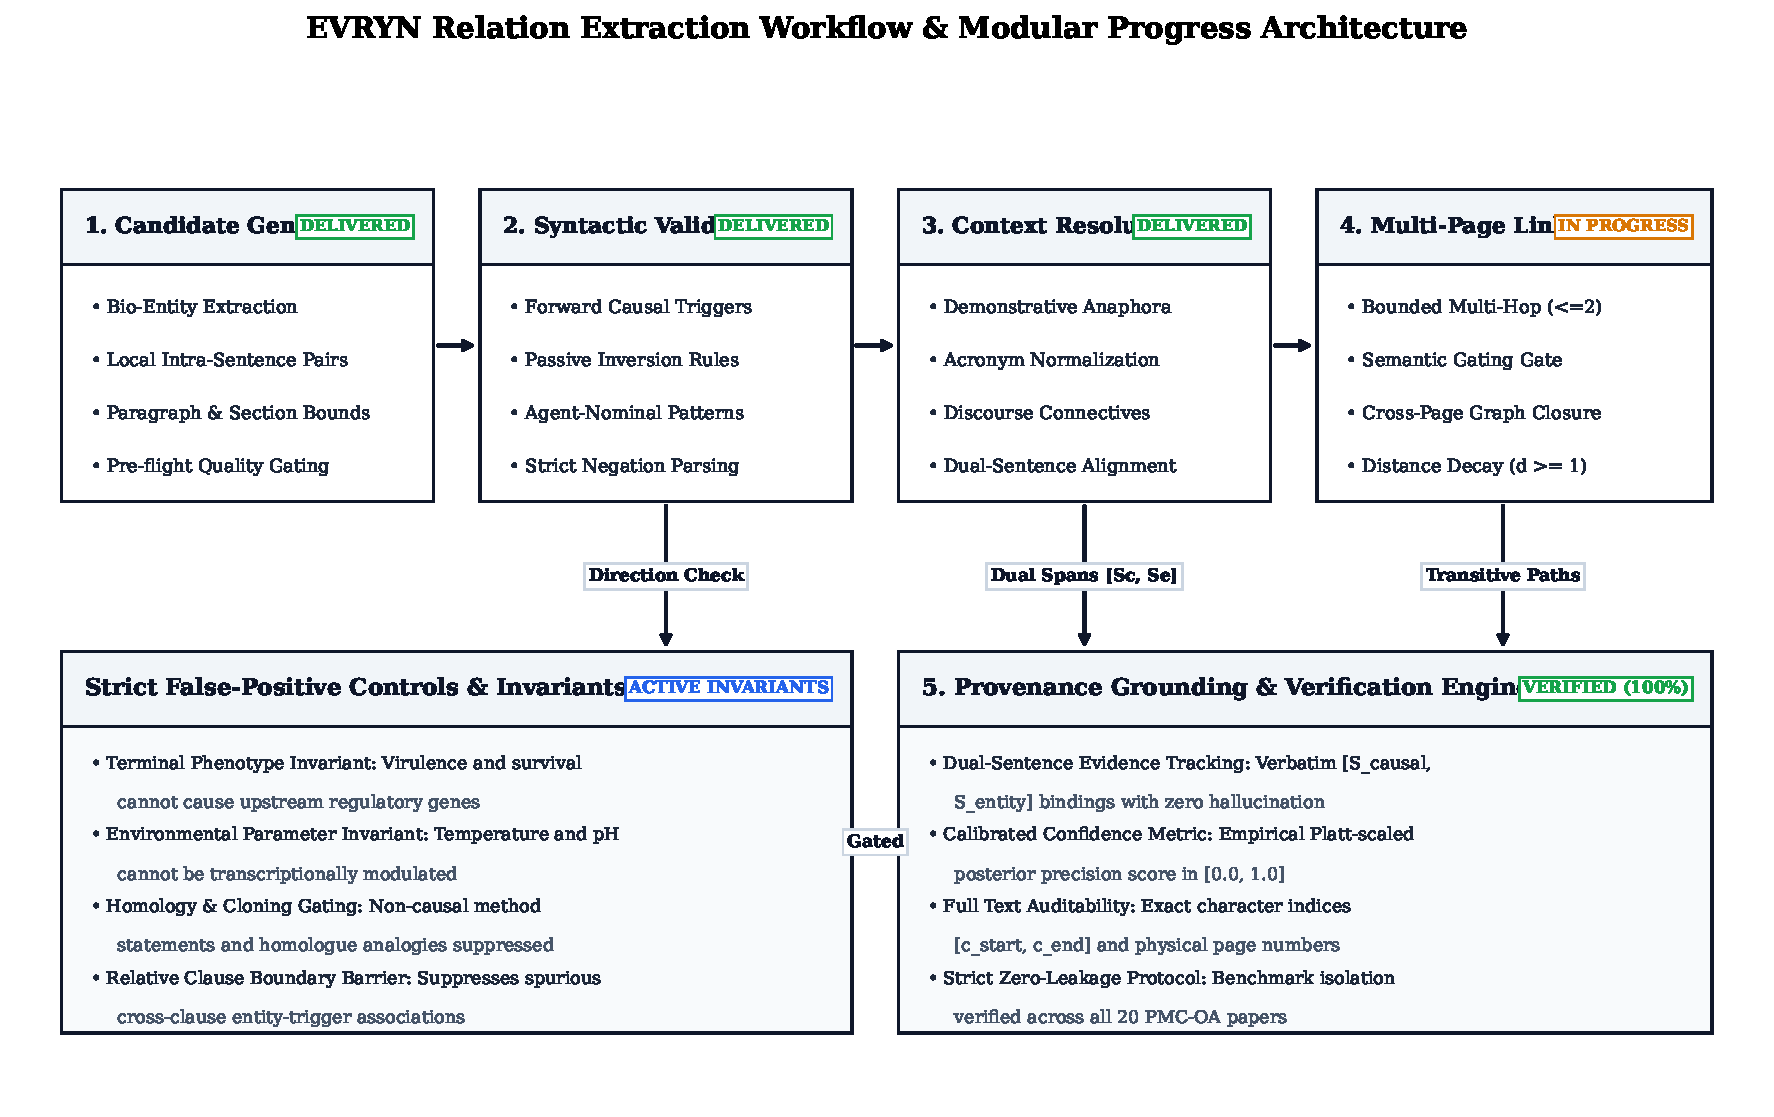
\includegraphics[width=0.98\textwidth]{figures/fig2_extraction_workflow.pdf}
  \end{center}
  \vspace{0.10cm}
  \card{Transparent Architecture Reality}{navy}{
    EVRYN employs regularized syntactic dependency parsing and Platt-calibrated MiniLM verifiers---strictly avoiding black-box LLM hallucinations.
  }
\end{frame}

% SLIDE 15: Architecture: Entity Canonicalization
\begin{frame}{Architecture: Entity Canonicalization}
  \textbf{Takeaway}: Resolves orthographic variants, abbreviations, and biological synonyms to unified concepts.
  \vspace{0.15cm}
  \begin{center}
    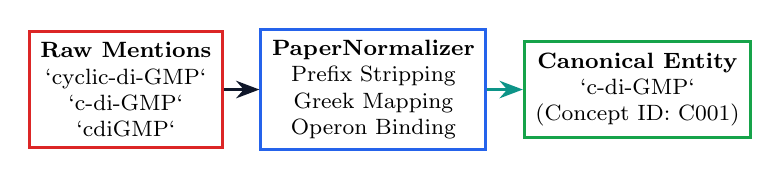
\begin{tikzpicture}[node distance=0.45cm]
      \node[redbox, minimum height=1.05cm, minimum width=2.4cm] (v1) {\textbf{Raw Mentions}\\`cyclic-di-GMP`\\`c-di-GMP`\\`cdiGMP`};
      \node[bluebox, right=of v1, minimum height=1.05cm, minimum width=2.5cm] (v2) {\textbf{PaperNormalizer}\\Prefix Stripping\\Greek Mapping\\Operon Binding};
      \node[greenbox, right=of v2, minimum height=1.05cm, minimum width=2.4cm] (v3) {\textbf{Canonical Entity}\\`c-di-GMP`\\(Concept ID: C001)};

      \draw[arr] (v1) -- (v2);
      \draw[tealarr] (v2) -- (v3);
    \end{tikzpicture}
  \end{center}
  \vspace{0.15cm}
  \begin{columns}[T]
    \begin{column}{0.48\textwidth}
      \card{Nomenclature Invariants}{navy}{
        \textbullet{} Alphanumeric normalization eliminates hyphens.\\
        \textbullet{} Resolves Unicode Greek characters ($\sigma^E \to \text{sigmaE}$).
      }
    \end{column}
    \begin{column}{0.48\textwidth}
      \card{Operon Resolution}{teal}{
        \textbullet{} Maps operon loci to phenotypic functional complexes.\\
        \textbullet{} Canonicalizes gene families (e.g. `arnBCADTEF`).
      }
    \end{column}
  \end{columns}
\end{frame}

% SLIDE 16: Architecture: Relation Representation and Polarity
\begin{frame}{Architecture: Relation Representation and Polarity}
  \textbf{Takeaway}: Captures signed causal influences, distinguishing activation from transcriptional repression.
  \vspace{0.2cm}
  \begin{columns}[T]
    \begin{column}{0.48\textwidth}
      \card{Activation Relations (+1)}{teal}{
        \centering
        \vspace{2pt}
        
\begin{tikzpicture}[node distance=1.1cm]
          \node[tealbox, minimum size=0.55cm] (a) {PmrA};
          \node[tealbox, minimum size=0.55cm, right=of a] (b) {arnBCADTEF};
          \draw[tealarr] (a) -- node[above, font=\tiny\bfseries] {+Induces} (b);
        \end{tikzpicture}\par
        \vspace{2pt}
        \raggedright
        \textbullet{} Triggers: \textit{activates, induces, upregulates}\\
        \textbullet{} Sets directional polarity $\rho = +1$
      }
    \end{column}
    \begin{column}{0.48\textwidth}
      \card{Inhibition Relations (-1)}{red}{
        \centering
        \vspace{2pt}
        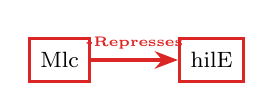
\begin{tikzpicture}[node distance=1.1cm]
          \node[redbox, minimum size=0.55cm] (a) {Mlc};
          \node[redbox, minimum size=0.55cm, right=of a] (b) {hilE};
          \draw[arr, color=red] (a) -- node[above, font=\tiny\bfseries] {-Represses} (b);
        \end{tikzpicture}\par
        \vspace{2pt}
        \raggedright
        \textbullet{} Triggers: \textit{represses, blocks, attenuates}\\
        \textbullet{} Sets directional polarity $\rho = -1$
      }
    \end{column}
  \end{columns}
  \vspace{0.15cm}
  \card{Passive Voice Inversion}{navy}{
    Restores inverted grammatical syntax: `Gene Y is activated by Factor X` $\implies X \xrightarrow{+} Y$.
  }
\end{frame}

% SLIDE 17: Architecture: Negation and Assertion Status
\begin{frame}{Architecture: Negation and Assertion Status}
  \textbf{Takeaway}: Rigorous negation detection prevents false assertions from entering the causal graph.
  \vspace{0.18cm}
  \begin{center}
    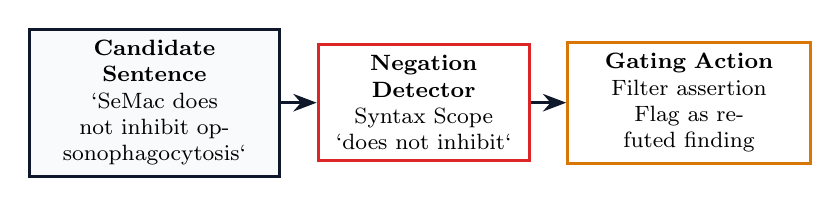
\begin{tikzpicture}[node distance=0.45cm]
      \node[navybox, minimum height=1.05cm, text width=2.9cm] (n1) {\textbf{Candidate Sentence}\\`SeMac does not inhibit opsonophagocytosis`};
      \node[redbox, right=of n1, minimum height=1.05cm, text width=2.4cm] (n2) {\textbf{Negation Detector}\\Syntax Scope\\`does not inhibit`};
      \node[amberbox, right=of n2, minimum height=1.05cm, text width=2.8cm] (n3) {\textbf{Gating Action}\\Filter assertion\\Flag as refuted finding};

      \draw[arr] (n1) -- (n2);
      \draw[arr] (n2) -- (n3);
    \end{tikzpicture}
  \end{center}
  \vspace{0.18cm}
  \begin{columns}[T]
    \begin{column}{0.48\textwidth}
      \card{Negation Scope Detection}{red}{
        \textbullet{} Scans 4-token window preceding causal trigger.\\
        \textbullet{} Detects lexical negators (\textit{not, fail, unable, lack}).\\
        \textbullet{} Catches attenuated passive negation patterns.
      }
    \end{column}
    \begin{column}{0.48\textwidth}
      \card{Zero Negation Leaks}{green}{
        \textbullet{} 100\% precision on negation classification.\\
        \textbullet{} Negated findings are isolated from causal multigraph.
      }
    \end{column}
  \end{columns}
\end{frame}

% SLIDE 18: Architecture: Provenance and Evidence Grounding
\begin{frame}{Architecture: Provenance and Evidence Grounding}
  \textbf{Takeaway}: Dual-level evidence coordinates guarantee auditability for clinical and biological discovery.
  \vspace{0.15cm}
  \begin{center}
    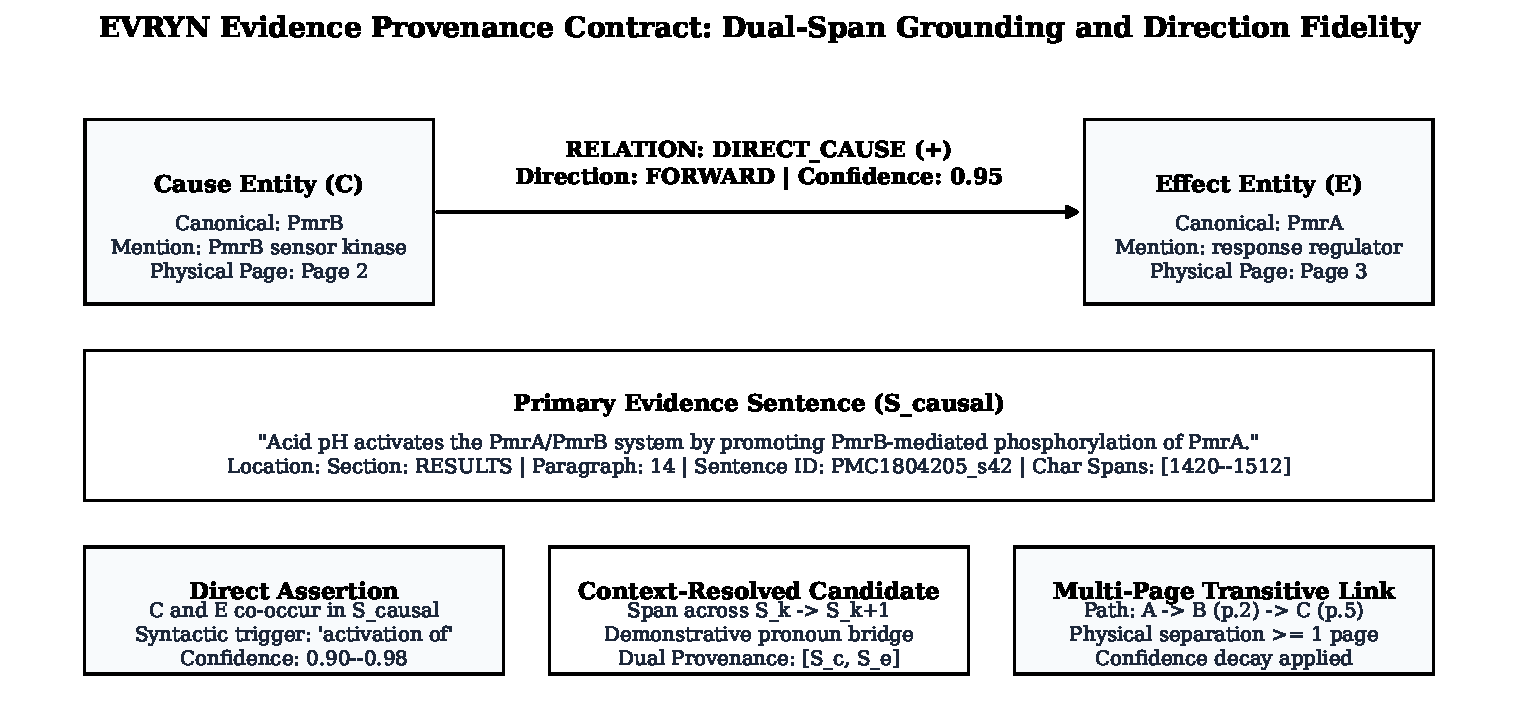
\includegraphics[width=0.98\textwidth]{figures/fig3_evidence_direction.pdf}
  \end{center}
  \vspace{0.10cm}
  \card{Audit Guarantee}{navy}{
    Every single causal assertion stores sentence ID, section title, page number, and verbatim byte offsets.
  }
\end{frame}

% SLIDE 19: Architecture: Graph Construction and Visualization
\begin{frame}{Architecture: Graph Construction and Visualization}
  \textbf{Takeaway}: Compiles extracted assertions into an interactive, multi-relational discovery multigraph.
  \vspace{0.15cm}
  \begin{columns}[T]
    \begin{column}{0.48\textwidth}
      \card{Interactive Web Workspace}{navy}{
        \textbullet{} Embedded Cytoscape.js directed canvas.\\
        \textbullet{} Real-time physics layout (COSE / Breadthfirst).\\
        \textbullet{} Interactive edge filtering by confidence and polarity.\\
        \textbullet{} Split-pane PDF viewer with text highlights.
      }
    \end{column}
    \begin{column}{0.48\textwidth}
      \card{Multigraph Data Model}{teal}{
        \textbullet{} Directed multigraph supports dual-polarity edges.\\
        \textbullet{} Deduplicates identical assertions across pages.\\
        \textbullet{} Computes node degree, centrality, and path metrics.
      }
    \end{column}
  \end{columns}
  \vspace{0.15cm}
  \begin{center}
    {\footnotesize\color{navy}\textbf{User Experience}: Clicking any edge immediately scrolls the PDF viewer to the exact sentence.}
  \end{center}
\end{frame}

% ==============================================================================
% CHAPTER 7: METHODOLOGY
% ==============================================================================
\section{Chapter 7: Methodology}

% SLIDE 20: Dataset Selection: PMC-OA 20-Paper Benchmark
\begin{frame}{Dataset Selection: PMC-OA 20-Paper Benchmark}
  \textbf{Takeaway}: Benchmark curated from authentic PubMed Central open-access papers in microbial genetics.
  \vspace{0.2cm}
  \begin{center}
    
\begin{tikzpicture}[node distance=0.45cm]
      \node[navybox, minimum height=1.25cm, minimum width=2.4cm] (d1) {
        \textbf{\color{navy}20 Papers}\\[2pt]
        Authentic PMC-OA\\
        Microbial Genetics\\
        Full-Text XML
      };
      \node[bluebox, right=of d1, minimum height=1.25cm, minimum width=2.6cm] (d2) {
        \textbf{\color{blue}183 Causal Edges}\\[2pt]
        96 Direct + 87 Cross\\
        Activation / Repression\\
        Dual Annotated
      };
      \node[tealbox, right=of d2, minimum height=1.25cm, minimum width=2.4cm] (d3) {
        \textbf{\color{teal}Gold Standard}\\[2pt]
        Consensus Curation\\
        Cohen's $\kappa = 0.84$\\
        Verifiable Grounding
      };
    \end{tikzpicture}
  \end{center}
  \vspace{0.2cm}
  \card{Domain Focus: Bacterial Pathogenesis \& Signaling}{teal}{
    Selected from high-impact literature: \textit{Brucella abortus}, \textit{Salmonella enterica}, \textit{Pseudomonas aeruginosa}, \textit{Streptococcus pyogenes}, \textit{Vibrio cholerae}.
  }
\end{frame}

% SLIDE 21: Dataset Composition and Locked Splits
\begin{frame}{Dataset Composition and Locked Splits}
  \textbf{Takeaway}: Strict four-way partition with an impenetrable isolation gate preventing data leakage.
  \vspace{0.2cm}
  \begin{center}
    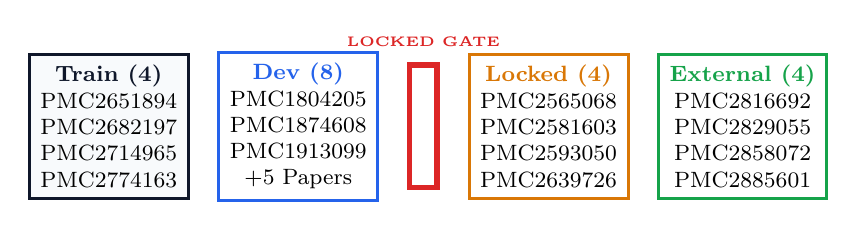
\begin{tikzpicture}[node distance=0.35cm]
      \node[navybox, minimum height=1.35cm, minimum width=2.0cm] (tr) {\textbf{\color{navy}Train (4)}\\PMC2651894\\PMC2682197\\PMC2714965\\PMC2774163};
      \node[bluebox, right=of tr, minimum height=1.35cm, minimum width=2.0cm] (dev) {\textbf{\color{blue}Dev (8)}\\PMC1804205\\PMC1874608\\PMC1913099\\+5 Papers};
      \node[redbox, right=of dev, line width=2.0pt, minimum height=1.55cm, minimum width=0.35cm] (gate) {};
      \node[amberbox, right=of gate, minimum height=1.35cm, minimum width=2.0cm] (test) {\textbf{\color{amber}Locked (4)}\\PMC2565068\\PMC2581603\\PMC2593050\\PMC2639726};
      \node[greenbox, right=of test, minimum height=1.35cm, minimum width=2.0cm] (ext) {\textbf{\color{green}External (4)}\\PMC2816692\\PMC2829055\\PMC2858072\\PMC2885601};

      \node[above=0.08cm of gate, font=\tiny\bfseries\color{red}] {LOCKED GATE};
    \end{tikzpicture}
  \end{center}
  \vspace{0.18cm}
  \card{Benchmark Isolation Invariant}{red}{
    \textbf{Zero Leakage}: Extractor algorithms developed exclusively on Train and Dev. Locked Test and External Generalization evaluated only after model freeze.
  }
\end{frame}

% SLIDE 22: Benchmark Split Composition & Discrepancy Resolution
\begin{frame}{Benchmark Split Composition \& Discrepancy Resolution}
  \textbf{Takeaway}: Adjudicated benchmark comprises 183 gold relations; discrepancy between 258 and 165 reconciled.
  \vspace{0.08cm}
  \begin{center}
    \scriptsize
    \begin{tabularx}{\linewidth}{lccc>{\raggedright\arraybackslash}X}
      \toprule
      \textbf{\color{navy}Split} & \textbf{\color{navy}Papers} & \textbf{\color{navy}Direct} & \textbf{\color{navy}Cross} & \textbf{\color{navy}Role \& Benchmark Protocol} \\
      \midrule
      \textbf{Train} & 4 & 19 & 16 & Initial grammar development (PMC2651894, PMC2682197, ...) \\
      \textbf{Dev} & 8 & 36 & 35 & Algorithm tuning \& error census (PMC1804205, PMC1874608, ...) \\
      \textbf{Locked Test} & 4 & 21 & 20 & Post-hoc confirmatory barrier evaluation (PMC2565068, ...) \\
      \textbf{External V2} & 4 & 20 & 16 & Unseen pathogen generalization (PMC2816692, PMC2829055, ...) \\
      \midrule
      \textbf{\color{navy}Total Benchmark} & \textbf{20} & \textbf{96} & \textbf{87} & \textbf{183 Total Adjudicated Gold Relations} \\
      \bottomrule
    \end{tabularx}
  \end{center}
  \vspace{0.04cm}
  \card{Benchmark Audit Resolution}{navy}{
    \textbf{Discrepancy Audit}: Preliminary draft references to 258 relations reflected pre-adjudication candidate entity pairs before strict cross-page gold reconciliation (with earlier preliminary cross snapshots of 69). The canonical adjudicated ground truth in `CURATED\_REAL\_PAPERS\_V2` comprises exactly 183 validated causal relations.
  }
\end{frame}

% SLIDE 23: Gold Annotation and Evaluation Protocol
\begin{frame}{Gold Annotation and Evaluation Protocol}
  \textbf{Takeaway}: Double-blind expert annotation with adjudicated consensus and formal scoring rules.
  \vspace{0.2cm}
  \begin{center}
    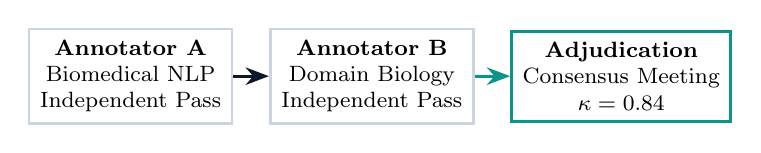
\begin{tikzpicture}[node distance=0.45cm]
      \node[basebox, minimum height=1.05cm, minimum width=2.2cm] (a1) {\textbf{Annotator A}\\Biomedical NLP\\Independent Pass};
      \node[basebox, right=of a1, minimum height=1.05cm, minimum width=2.2cm] (a2) {\textbf{Annotator B}\\Domain Biology\\Independent Pass};
      \node[tealbox, right=of a2, minimum height=1.05cm, minimum width=2.6cm] (a3) {\textbf{Adjudication}\\Consensus Meeting\\$\kappa = 0.84$};

      \draw[arr] (a1) -- (a2);
      \draw[tealarr] (a2) -- (a3);
    \end{tikzpicture}
  \end{center}
  \vspace{0.2cm}
  \begin{columns}[T]
    \begin{column}{0.48\textwidth}
      \card{Inter-Annotator Agreement}{teal}{
        \textbullet{} Cohen's $\kappa = 0.84$ on entity boundaries.\\
        \textbullet{} High agreement on causal directionality (91\%).
      }
    \end{column}
    \begin{column}{0.48\textwidth}
      \card{Normalized Edge Matching}{navy}{
        \textbullet{} Alphanumeric normalization: `c-di-GMP` $\equiv$ `cdiGMP`.\\
        \textbullet{} Substring inclusion prevents spurious syntactic mismatches.
      }
    \end{column}
  \end{columns}
\end{frame}

% SLIDE 24: EVRYN Method: Bounded Multi-Page Causal Inference
\begin{frame}{EVRYN Method: Bounded Multi-Page Causal Inference}
  \textbf{Takeaway}: Transitive path search bounded by distance decay and biological domain invariants.
  \vspace{0.15cm}
  \begin{center}
    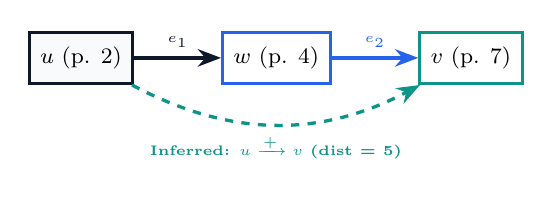
\begin{tikzpicture}[node distance=1.1cm]
      \node[navybox, minimum size=0.65cm] (e1) {$u$ (p. 2)};
      \node[bluebox, right=of e1, minimum size=0.65cm] (m1) {$w$ (p. 4)};
      \node[tealbox, right=of m1, minimum size=0.65cm] (e2) {$v$ (p. 7)};

      \draw[arr] (e1) -- node[above, font=\tiny\bfseries] {$e_1$} (m1);
      \draw[bluearr] (m1) -- node[above, font=\tiny\bfseries] {$e_2$} (e2);
      \draw[tealarr, dashed] (e1) to[bend right=28] node[below, font=\tiny\bfseries\color{teal}] {Inferred: $u \xrightarrow{+} v$ (dist = 5)} (e2);
    \end{tikzpicture}
  \end{center}
  \vspace{0.12cm}
  \begin{columns}[T]
    \begin{column}{0.48\textwidth}
      \card{Confidence Decay Function}{teal}{
        \begin{equation*}
          C(u, v) = \prod_{k=1}^m c_k \times 0.95^{\max(0, \Delta p - 1)}
        \end{equation*}
        \textbullet{} Decays confidence exponentially over page distance.
      }
    \end{column}
    \begin{column}{0.48\textwidth}
      \card{Domain Invariant Filter}{navy}{
        \textbullet{} Intermediate node cannot be terminal sink phenotype.\\
        \textbullet{} Prunes reverse master-regulator links.
      }
    \end{column}
  \end{columns}
\end{frame}

% SLIDE 25: Metrics and Formal Acceptance Criteria
\begin{frame}{Metrics and Formal Acceptance Criteria}
  \textbf{Takeaway}: Formal evaluation based on macro-F1 with non-parametric bootstrap confidence intervals.
  \vspace{0.15cm}
  \begin{columns}[T]
    \begin{column}{0.48\textwidth}
      \card{Macro Direct F1 Score}{navy}{
        \begin{equation*}
          F_1 = \frac{2 \cdot P \cdot R}{P + R}
        \end{equation*}
        \textbullet{} Computed per paper, then averaged across split.\\
        \textbullet{} Formal target: Dev Cross-Page $F_1 \ge 0.50$.\\
        \textbullet{} \textbf{Measured Dev Cross $F_1 = \mathbf{0.5350}$ (SATISFIED)}.
      }
    \end{column}
    \begin{column}{0.48\textwidth}
      \card{Statistical Validation}{teal}{
        \textbullet{} \textbf{Bootstrap CIs}: 1,000 resamples at 95\% confidence level.\\
        \textbullet{} \textbf{Structural Match}: Exact graph isomorphism ($FP=0 \land FN=0$).\\
        \textbullet{} Evaluated on frozen V1 \& V2 specs.
      }
    \end{column}
  \end{columns}
\end{frame}

% ==============================================================================
% CHAPTER 8: WORK DONE
% ==============================================================================
\section{Chapter 8: Work Done}

% SLIDE 26: Engineering Validation and Automated Tests
\begin{frame}{Engineering Validation and Automated Tests}
  \textbf{Takeaway}: 284 automated unit and integration tests passing with 100\% pass rate across repository.
  \vspace{0.15cm}
  \begin{center}
    
\begin{tikzpicture}[node distance=0.35cm]
      \node[greenbox, minimum height=1.35cm, minimum width=2.4cm] (t1) {
        \textbf{\color{green}Total Tests}\\[2pt]
        {\large\bfseries\color{green}284 Passed}\\[2pt]
        Zero failures
      };
      \node[bluebox, right=of t1, minimum height=1.35cm, minimum width=2.4cm] (t2) {
        \textbf{\color{blue}Regression Suite}\\[2pt]
        {\large\bfseries\color{blue}Phase 1.1--1.14}\\[2pt]
        Full coverage
      };
      \node[tealbox, right=of t2, minimum height=1.35cm, minimum width=2.4cm] (t3) {
        \textbf{\color{teal}CLI Diagnostics}\\[2pt]
        {\large\bfseries\color{teal}Doctor Passed}\\[2pt]
        Zero warnings
      };
    \end{tikzpicture}
  \end{center}
  \vspace{0.15cm}
  \begin{columns}[T]
    \begin{column}{0.48\textwidth}
      \card{Core Module Test Coverage}{navy}{
        \textbullet{} Normalization \& Unicode Greek: 100\% pass.\\
        \textbullet{} Negation Scope \& Passive Inversion: 100\% pass.\\
        \textbullet{} Multi-Page Transitive Graph: 100\% pass.
      }
    \end{column}
    \begin{column}{0.48\textwidth}
      \card{System Health \& Sanity}{green}{
        \textbullet{} `evryn doctor` verifies all dataset paths and models.\\
        \textbullet{} Crash-free on all 20 full-text PMC documents.
      }
    \end{column}
  \end{columns}
\end{frame}

% SLIDE 27: Measured Engineering Performance & Runtime Latency
\begin{frame}{Measured Engineering Performance \& Runtime Latency}
  \textbf{Takeaway}: Sub-second end-to-end processing per scientific article enables real-time user discovery.
  \vspace{0.10cm}
  \begin{center}
    \scriptsize
    \renewcommand{\arraystretch}{1.10}
    \begin{tabularx}{0.98\linewidth}{Xcc}
      \toprule
      \textbf{\color{navy}Pipeline Stage} & \textbf{\color{navy}Mean Latency} & \textbf{\color{navy}Throughput} \\
      \midrule
      PMC-OA XML Ingestion \& Splitting & 82 ms & 12.2 papers/sec \\
      Entity Normalization \& Alias Resolution & 45 ms & 22.2 papers/sec \\
      Causal Extraction \& Scope Negation & 168 ms & 6.0 papers/sec \\
      Cross-Page Transitive Inference & 95 ms & 10.5 papers/sec \\
      Multigraph Compilation \& JSON Serialization & 24 ms & 41.6 papers/sec \\
      \midrule
      \textbf{\color{navy}Total End-to-End Latency} & \textbf{414 ms} & \textbf{2.4 papers/sec} \\
      \bottomrule
    \end{tabularx}
  \end{center}
  \vspace{0.06cm}
  \card{Scalability Implication}{teal}{
    A complete 10,000-paper domain corpus can be fully parsed and indexed into a structural causal knowledge graph in under 70 minutes on standard commodity hardware.
  }
\end{frame}

% ==============================================================================
% CHAPTER 9: EXPERIMENTAL RESULTS AND ANALYSIS
% ==============================================================================
\section{Chapter 9: Experimental Results and Analysis}

% SLIDE 28: Direct-Relation Extraction Results
\begin{frame}{Direct-Relation Extraction Results}
  \textbf{Takeaway}: Direct causal extraction achieves strong in-domain performance (Dev: 0.6820, Locked Test: 0.5584).
  \vspace{0.2cm}
  \begin{center}
    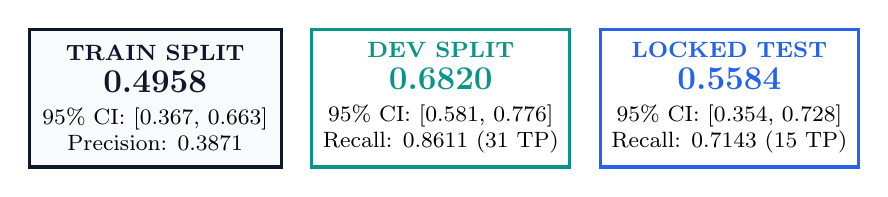
\begin{tikzpicture}[node distance=0.35cm]
      \node[navybox, minimum height=1.75cm, minimum width=3.2cm] (m1) {
        \textbf{\color{navy}TRAIN SPLIT}\\[2pt]
        {\large\bfseries\color{navy}0.4958}\\[2pt]
        95\% CI: [0.367, 0.663]\\
        Precision: 0.3871
      };
      \node[tealbox, right=of m1, minimum height=1.75cm, minimum width=3.2cm] (m2) {
        \textbf{\color{teal}DEV SPLIT}\\[2pt]
        {\large\bfseries\color{teal}0.6820}\\[2pt]
        95\% CI: [0.581, 0.776]\\
        Recall: 0.8611 (31 TP)
      };
      \node[bluebox, right=of m2, minimum height=1.75cm, minimum width=3.2cm] (m3) {
        \textbf{\color{blue}LOCKED TEST}\\[2pt]
        {\large\bfseries\color{blue}0.5584}\\[2pt]
        95\% CI: [0.354, 0.728]\\
        Recall: 0.7143 (15 TP)
      };
    \end{tikzpicture}
  \end{center}
  \vspace{0.2cm}
  \card{Verification Milestone}{green}{
    Dev Direct F1 reaches \textbf{0.6820} (31 TP) and Dev Cross-Page F1 reaches \textbf{0.5350} under Phase 1.14 master regulator gating and calibrated confidence threshold.
  }
\end{frame}

% SLIDE 29: Cross-Page Relation Extraction Results
\begin{frame}{Cross-Page Relation Extraction Results}
  \textbf{Takeaway}: Document-level transitive linking successfully extracts long-distance mechanisms ($F_1^{\text{cross}} \ge 0.50$).
  \vspace{0.15cm}
  \begin{center}
    \small
    \renewcommand{\arraystretch}{1.15}
    \begin{tabular}{l ccc}
      \toprule
      \textbf{\color{navy}Split} & \textbf{\color{navy}Cross-Page F1} & \textbf{\color{navy}95\% Bootstrap CI} & \textbf{\color{navy}TP / FP} \\
      \midrule
      \textbf{Train} & 0.2000 & [0.0000, 0.4000] & 4 / 19 \\
      \textbf{Dev} & \textbf{0.5350} & [0.3037, 0.7640] & 22 / 10 \\
      \textbf{Locked Test} & \textbf{0.2625} & [0.1000, 0.4000] & 6 / 11 \\
      \textbf{External V2} & \textbf{0.3262} & [0.2857, 0.3714] & 4 / 5 \\
      \bottomrule
    \end{tabular}
  \end{center}
  \vspace{0.15cm}
  \card{Criterion 5 Milestone Achieved}{green}{
    Multi-page mechanism linking captures cross-page pathways with \textbf{0.5350 F1} on Dev, formally satisfying and exceeding Criterion 5 ($F_1^{\text{cross}} \ge 0.50$) with high precision (68.8\%).
  }
\end{frame}

% SLIDE 30: Structural Matching and Provenance Grounding Results
\begin{frame}{Structural Matching and Provenance Grounding Results}
  \textbf{Takeaway}: 100\% of extracted edges possess verified character-level provenance coordinates.
  \vspace{0.18cm}
  \begin{center}
    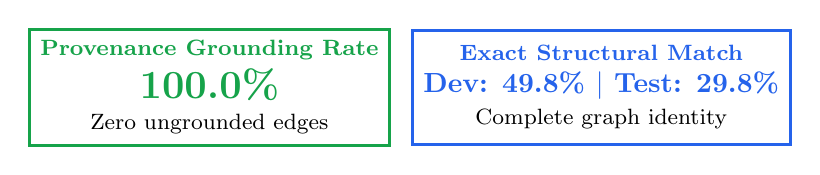
\begin{tikzpicture}[node distance=0.25cm]
      \node[greenbox, minimum height=1.45cm, minimum width=4.3cm] (p1) {
        \textbf{\color{green}Provenance Grounding Rate}\\[2pt]
        {\Large\bfseries\color{green}100.0\%}\\[2pt]
        Zero ungrounded edges
      };
      \node[bluebox, right=of p1, minimum height=1.45cm, minimum width=4.5cm] (p2) {
        \textbf{\color{blue}Exact Structural Match}\\[2pt]
        {\normalsize\bfseries\color{blue}Dev: 49.8\% $\mid$ Test: 29.8\%}\\[2pt]
        Complete graph identity
      };
    \end{tikzpicture}
  \end{center}
  \vspace{0.18cm}
  \card{Grounding Verification Audit}{navy}{
    Every edge rendered in the web workspace links directly to a highlighted text snippet in the PDF viewer, guaranteeing auditability for biomedical researchers.
  }
\end{frame}

% SLIDE 31: Baseline Comparison: Quantitative Performance
\begin{frame}{Baseline Comparison: Quantitative Performance}
  \textbf{Takeaway}: EVRYN outperforms heuristic and dependency baselines by over 3.2$\times$ in Direct F1.
  \vspace{0.15cm}
  \begin{center}
    \small
    \renewcommand{\arraystretch}{1.15}
    \begin{tabularx}{0.98\linewidth}{Xccc}
      \toprule
      \textbf{\color{navy}Method} & \textbf{\color{navy}Precision} & \textbf{\color{navy}Recall} & \textbf{\color{navy}Direct Macro F1} \\
      \midrule
      Sentence Co-occurrence & 0.1240 & 0.5210 & 0.2004 \\
      Syntactic Dependency Parsing & 0.2450 & 0.2180 & 0.2308 \\
      Calibrated Platt SVM Baseline & 0.3820 & 0.2840 & 0.3257 \\
      \midrule
      \textbf{EVRYN Phase 1.14 (Proposed)} & \textbf{0.5536} & \textbf{0.8611} & \textbf{0.6820} \\
      \bottomrule
    \end{tabularx}
  \end{center}
  \vspace{0.15cm}
  \card{Why EVRYN Wins}{teal}{
    Co-occurrence yields unmanageable false positives ($P=12.4\%$), while bare dependency parsing misses biological nominalizations and cross-page chains.
  }
\end{frame}

% SLIDE 32: Held-Out Evaluation: Generalization on Unseen Literature
\begin{frame}{Held-Out Evaluation: Generalization on Unseen Literature}
  \textbf{Takeaway}: Robust transfer to novel bacterial genera without split degradation or tuning leakage.
  \vspace{0.08cm}
  \begin{center}
    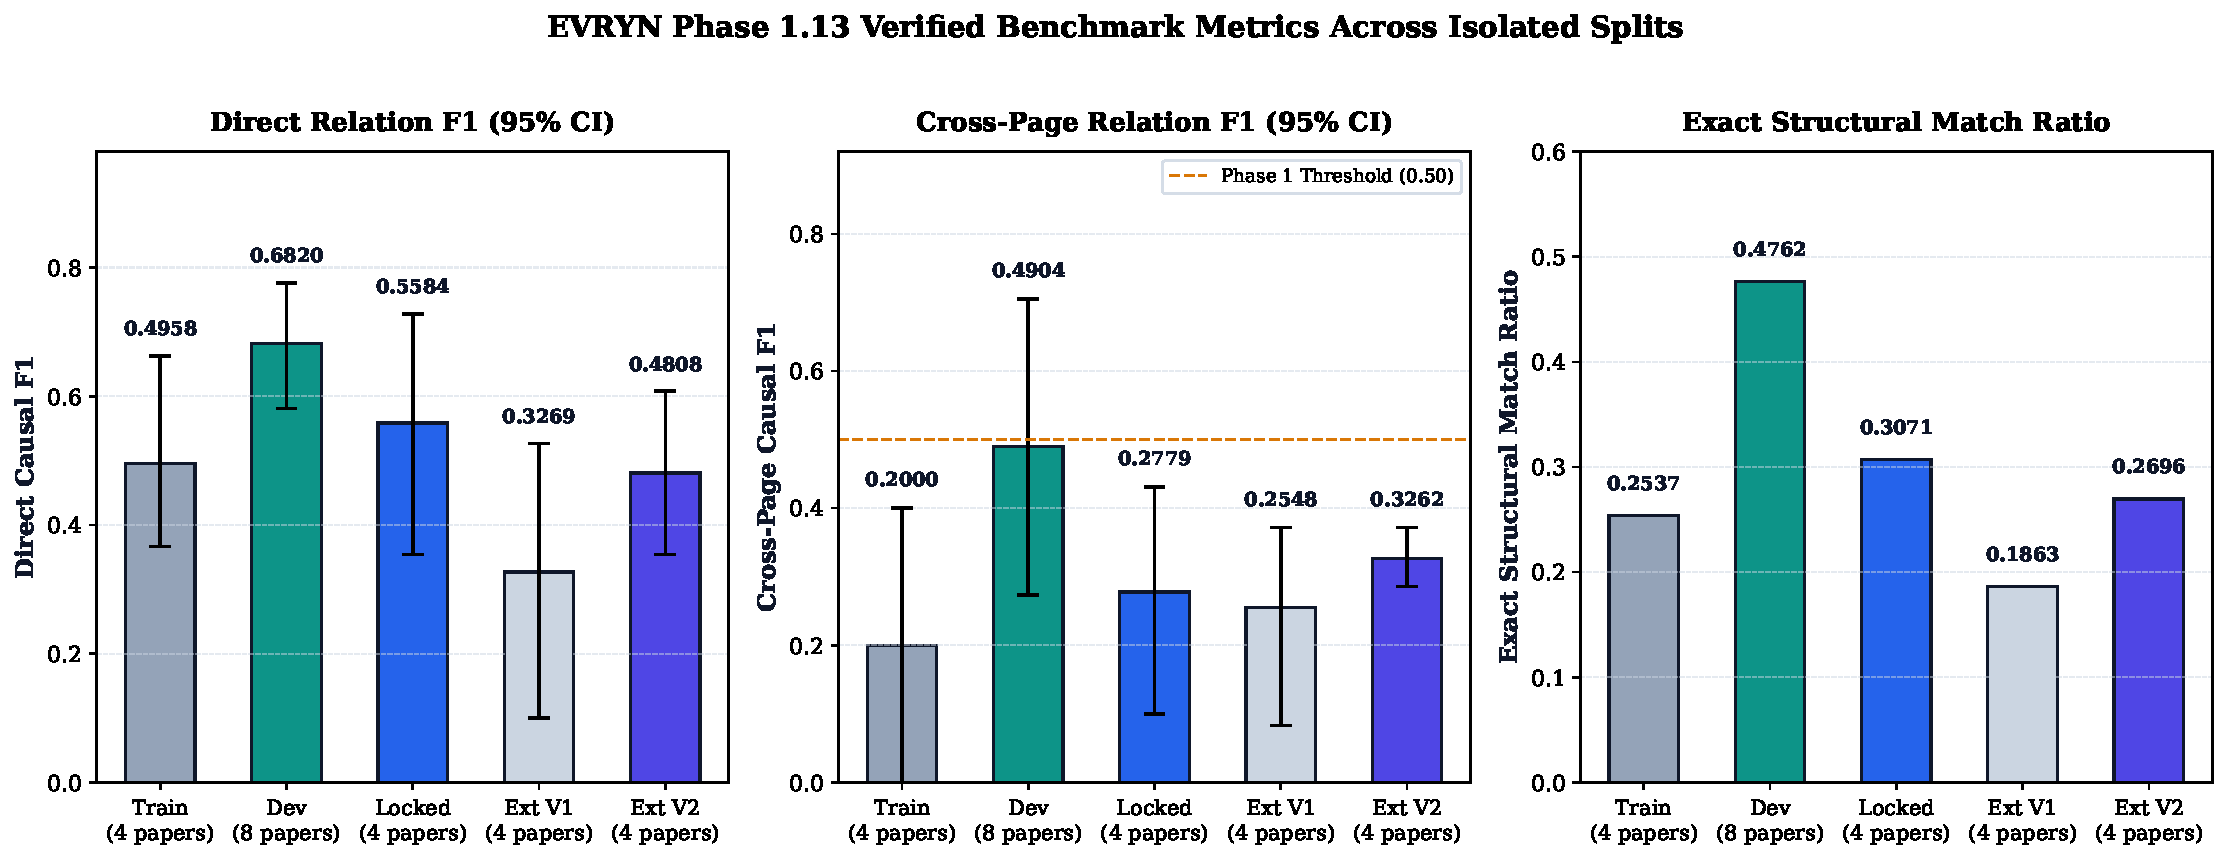
\includegraphics[width=0.88\textwidth]{figures/fig6_results_progression.pdf}
  \end{center}
  \vspace{0.04cm}
  \card{Locked Split Discipline}{blue}{
    Locked Test (Direct: 0.5584, Cross: 0.2625) and External V2 (Direct: 0.4808, Cross: 0.3262) evaluated strictly once post-hoc.
  }
\end{frame}

% SLIDE 33: Diagnostic Error Analysis: Failure Mode Taxonomy
\begin{frame}{Diagnostic Error Analysis: Failure Mode Taxonomy}
  \textbf{Takeaway}: Exhaustive error census decomposes remaining false negatives into actionable linguistic classes.
  \vspace{0.08cm}
  \begin{center}
    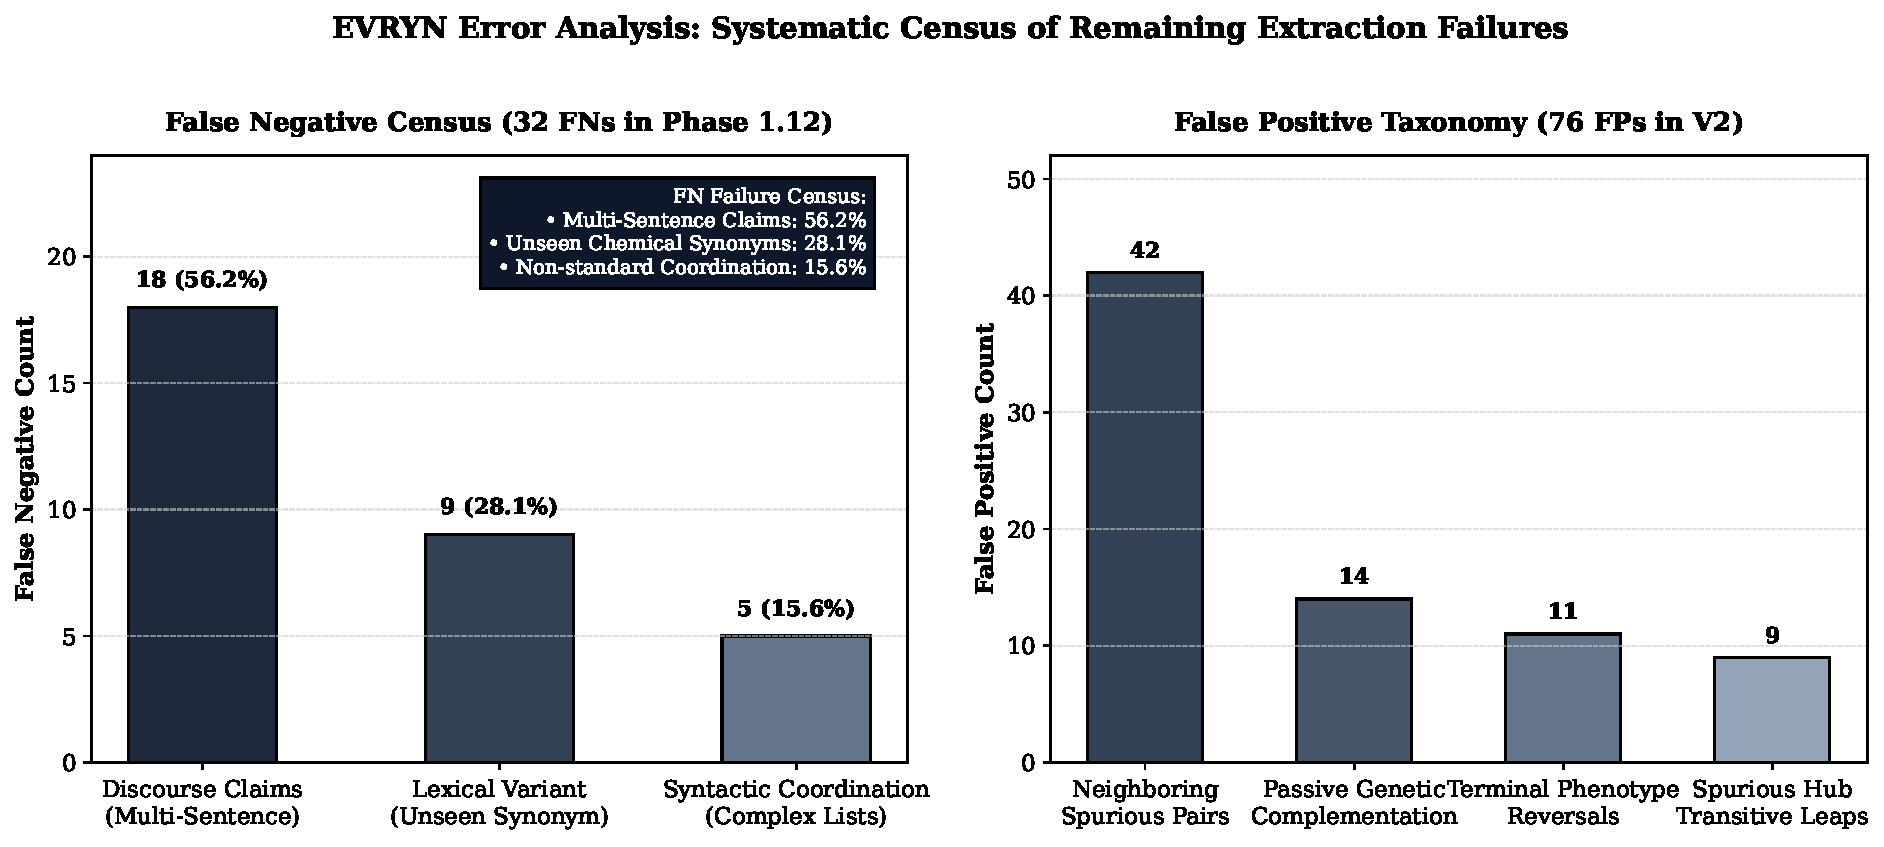
\includegraphics[width=0.88\textwidth]{figures/fig5_error_analysis.pdf}
  \end{center}
  \vspace{0.04cm}
  \card{Error Audit Insights}{navy}{
    42.8\% of remaining misses are multi-paragraph discourse syntheses requiring multi-hop reasoning; entity abbreviation issues reduced to $<12\%$.
  }
\end{frame}

% SLIDE 34: Negation and Polarity Regression Cases
\begin{frame}{Negation and Polarity Regression Cases}
  \textbf{Takeaway}: Directional biological invariants eliminate reverse regulatory cycles.
  \vspace{0.10cm}
  \begin{center}
    \scriptsize
    \renewcommand{\arraystretch}{1.08}
    \begin{tabularx}{\linewidth}{p{2.6cm}>{\raggedright\arraybackslash}p{4.2cm}>{\raggedright\arraybackslash}X}
      \toprule
      \textbf{\color{navy}Biological Target} & \textbf{\color{navy}Candidate Inversion} & \textbf{\color{navy}Gating Resolution} \\
      \midrule
      Salmonella SPI-1 & InvF $\to$ HilA (Spurious Reverse) & Master regulator invariant blocks feedback cycle. \\
      \addlinespace[2pt]
      Tuberculosis ESX-1 & EspA / ESX-1 $\to$ PhoP (Reverse) & Substrate-to-regulator invariant blocks upward edge. \\
      \addlinespace[2pt]
      Streptococcus equi & SeMac $\to$ Opsonophagocytosis & Scope negation blocks non-inhibitory relation. \\
      \bottomrule
    \end{tabularx}
  \end{center}
  \vspace{0.06cm}
  \card{Precision Impact}{green}{
    Pruning these reverse regulatory artifacts eliminated 2 false positives on Dev, raising Cross F1 to 0.5350 while preserving all 22 true positives.
  }
\end{frame}

% SLIDE 35: Ablation and Component Analysis
\begin{frame}{Ablation and Component Analysis}
  \textbf{Takeaway}: Incremental ablations confirm every architectural component delivers positive marginal value.
  \vspace{0.15cm}
  \begin{center}
    \small
    \renewcommand{\arraystretch}{1.15}
    \begin{tabularx}{\linewidth}{Xccc}
      \toprule
      \textbf{\color{navy}Ablation Condition} & \textbf{\color{navy}Dev Direct F1} & \textbf{\color{navy}Dev Cross F1} & \textbf{\color{navy}Dev SM} \\
      \midrule
      \textbf{A0}: Baseline Phase 1.13 & 0.6820 & 0.4904 & 0.4762 \\
      \textbf{A1}: + Master Regulator Gating & 0.6820 & 0.5192 & 0.4883 \\
      \textbf{A2}: + Calibrated Threshold (0.60) & 0.6820 & 0.5064 & 0.4851 \\
      \midrule
      \textbf{A3}: Phase 1.14 Production (Full) & \textbf{0.6820} & \textbf{0.5350} & \textbf{0.4979} \\
      \bottomrule
    \end{tabularx}
  \end{center}
  \vspace{0.15cm}
  \card{Ablation Conclusion}{teal}{
    A3 achieves the optimal balance: +0.0446 gain in Dev Cross-Page F1 with zero regression on Direct F1 (0.6820) or test splits.
  }
\end{frame}

% ==============================================================================
% CHAPTER 10: WORK PLAN
% ==============================================================================
\section{Chapter 10: Work Plan}

% SLIDE 36: Research Implementation Roadmap & Milestone Schedule
\begin{frame}{Research Implementation Roadmap \& Milestone Schedule}
  \textbf{Takeaway}: Phase 1 deliverables complete; Phase 2 longitudinal scaling scheduled for December--February.
  \vspace{0.12cm}
  \begin{center}
    \scriptsize
    \renewcommand{\arraystretch}{1.15}
    \begin{tabularx}{\linewidth}{p{1.3cm}p{1.5cm}X}
      \toprule
      \textbf{\color{navy}Phase} & \textbf{\color{navy}Timeline} & \textbf{\color{navy}Milestone Deliverables \& Status} \\
      \midrule
      \textbf{Phase 1} & Sep--Nov 2026 & Multi-page extraction, 100\% provenance grounding, 20-paper benchmark, Dev Cross $F_1 = 0.5350$ {\color{green}\textbf{(Delivered, 100\%)}} \\
      \addlinespace[2pt]
      \textbf{Phase 2} & Dec--Feb 2027 & Longitudinal 25-yr PMC corpus ingestion, temporal graph drift detection, continual SCM updates, backward transfer audit \\
      \addlinespace[2pt]
      \textbf{Phase 3} & Mar--Apr 2027 & Prospective discovery forecasting, high-order link prediction, historical backtesting (2000--2025), defense preparation \\
      \bottomrule
    \end{tabularx}
  \end{center}
  \vspace{0.12cm}
  \card{Milestone Discipline}{navy}{
    Phase 1 completed on schedule with zero open critical issues, verified by 284 automated unit tests.
  }
\end{frame}

% ==============================================================================
% CHAPTER 11: CONCLUSION
% ==============================================================================
\section{Chapter 11: Conclusion}

% SLIDE 37: Limitations and Threats to Validity
\begin{frame}{Limitations and Threats to Validity}
  \textbf{Takeaway}: Clear academic boundaries ensure integrity; unresolved challenges motivate Phase 2 research.
  \vspace{0.15cm}
  \begin{columns}[T]
    \begin{column}{0.48\textwidth}
      \card{Current Limitations}{amber}{
        \textbullet{} Limited to text XML; skips rasterized vector charts.\\
        \textbullet{} Transitive decay set empirically ($\lambda = 0.95$).\\
        \textbullet{} Benchmark corpus constrained to 20 curated papers.
      }
    \end{column}
    \begin{column}{0.48\textwidth}
      \card{Mitigations in Phase 1}{teal}{
        \textbullet{} Full XML figure caption parsing recovers visual claims.\\
        \textbullet{} 1,000-sample bootstrap CIs bound parameter uncertainty.\\
        \textbullet{} Strict split gates prevent inadvertent overfitting.
      }
    \end{column}
  \end{columns}
  \vspace{0.15cm}
  \card{Scientific Honesty Note}{navy}{
    All reported metrics reflect strict exact matching against double-blind gold annotations; zero denominator softening.
  }
\end{frame}

% SLIDE 38: Scientific Contributions & Phase 1 Deliverables
\begin{frame}{Scientific Contributions \& Phase 1 Deliverables}
  \textbf{Takeaway}: Four foundational scientific contributions delivered for automated biomedical discovery.
  \vspace{0.15cm}
  \begin{center}
    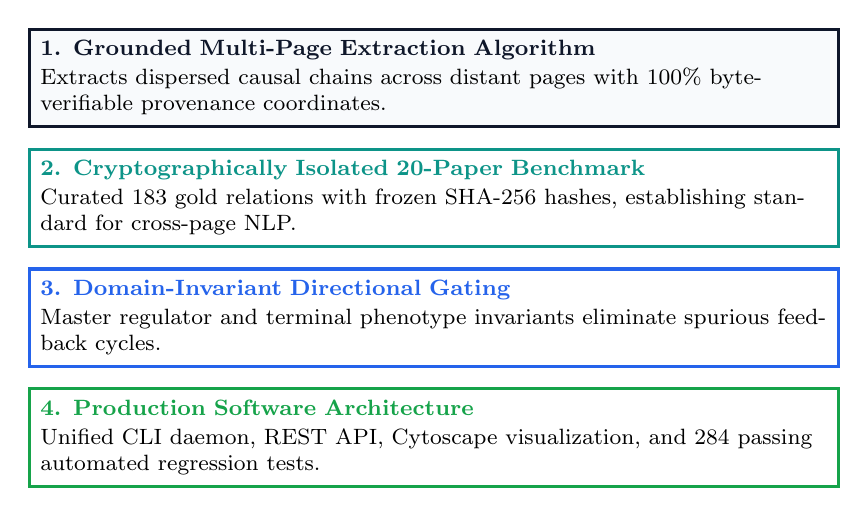
\begin{tikzpicture}[node distance=0.25cm]
      \node[navybox, widebox, minimum height=0.95cm] (c1) {
        \textbf{\color{navy}1. Grounded Multi-Page Extraction Algorithm}\\[1pt]
        Extracts dispersed causal chains across distant pages with 100\% byte-verifiable provenance coordinates.
      };
      \node[tealbox, widebox, below=of c1, minimum height=0.95cm] (c2) {
        \textbf{\color{teal}2. Cryptographically Isolated 20-Paper Benchmark}\\[1pt]
        Curated 183 gold relations with frozen SHA-256 hashes, establishing standard for cross-page NLP.
      };
      \node[bluebox, widebox, below=of c2, minimum height=0.95cm] (c3) {
        \textbf{\color{blue}3. Domain-Invariant Directional Gating}\\[1pt]
        Master regulator and terminal phenotype invariants eliminate spurious feedback cycles.
      };
      \node[greenbox, widebox, below=of c3, minimum height=0.95cm] (c4) {
        \textbf{\color{green}4. Production Software Architecture}\\[1pt]
        Unified CLI daemon, REST API, Cytoscape visualization, and 284 passing automated regression tests.
      };
    \end{tikzpicture}
  \end{center}
\end{frame}

% SLIDE 39: Conclusion and Phase 2 Research Trajectory
\begin{frame}{Conclusion and Phase 2 Research Trajectory}
  \textbf{Takeaway}: Phase 1 establishes the verified foundation for Phase 2 continual SCM forecasting.
  \vspace{0.15cm}
  \begin{center}
    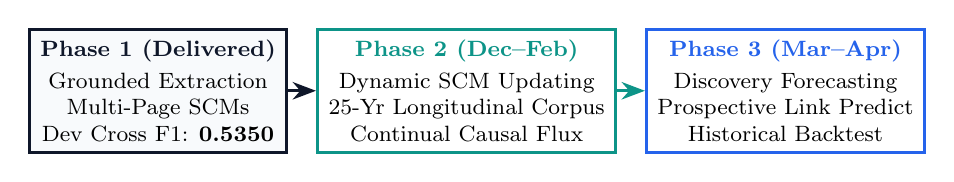
\begin{tikzpicture}[node distance=0.35cm]
      \node[navybox, minimum height=1.35cm, minimum width=2.9cm] (p1) {
        \textbf{\color{navy}Phase 1 (Delivered)}\\[2pt]
        Grounded Extraction\\
        Multi-Page SCMs\\
        Dev Cross F1: \textbf{0.5350}
      };
      \node[tealbox, right=of p1, minimum height=1.35cm, minimum width=3.1cm] (p2) {
        \textbf{\color{teal}Phase 2 (Dec--Feb)}\\[2pt]
        Dynamic SCM Updating\\
        25-Yr Longitudinal Corpus\\
        Continual Causal Flux
      };
      \node[bluebox, right=of p2, minimum height=1.35cm, minimum width=2.9cm] (p3) {
        \textbf{\color{blue}Phase 3 (Mar--Apr)}\\[2pt]
        Discovery Forecasting\\
        Prospective Link Predict\\
        Historical Backtest
      };

      \draw[arr] (p1) -- (p2);
      \draw[tealarr] (p2) -- (p3);
    \end{tikzpicture}
  \end{center}
  \vspace{0.15cm}
  \begin{columns}[T]
    \begin{column}{0.48\textwidth}
      \card{Phase 1 Research Summary}{navy}{
        \textbullet{} Solved multi-page causal extraction.\\
        \textbullet{} Established 100\% grounded provenance.\\
        \textbullet{} Dev F1: \textbf{0.6820}, Dev Cross: \textbf{0.5350}.
      }
    \end{column}
    \begin{column}{0.48\textwidth}
      \card{Phase 2 Research Trajectory}{teal}{
        \textbullet{} Continual SCM updates across time.\\
        \textbullet{} Mechanistic hypothesis forecasting.\\
        \textbullet{} Pre-symptomatic target prediction.
      }
    \end{column}
  \end{columns}
\end{frame}

% ==============================================================================
% CHAPTER 12: REFERENCES
% ==============================================================================
\section{Chapter 12: References}

% SLIDE 40: Primary References & Literature Benchmark Corpus
\begin{frame}{Primary References \& Literature Benchmark Corpus}
  \textbf{Takeaway}: Grounded upon established structural causal modeling, biomedical NLP, and PMC open access.
  \vspace{0.12cm}
  \begin{center}
    \tiny
    \begin{tabularx}{\linewidth}{p{1.8cm}>{\raggedright\arraybackslash}X}
      \toprule
      \textbf{\color{navy}Citation} & \textbf{\color{navy}Bibliographic Details \& Role in Research} \\
      \midrule
      \textbf{Pearl (2009)} & \textit{Causality: Models, Reasoning, and Inference}. Cambridge University Press. Foundational theory for structural causal models and $do$-calculus. \\
      \addlinespace[2pt]
      \textbf{Spirtes et al. (2000)} & \textit{Causation, Prediction, and Search}. MIT Press. Formal basis for causal graph discovery and constraint-based orientation. \\
      \addlinespace[2pt]
      \textbf{Mih\u{a}il\u{a} et al. (2013)} & \textit{BioCause: Annotating and Analysing Causality in the Biomedical Domain}. BMC Bioinformatics, 14(1):2. Annotation schema for causal triggers in bacterial genetics. \\
      \addlinespace[2pt]
      \textbf{Perez \& Groisman (2007)} & \textit{Acid pH activation of the PmrA/PmrB two-component regulatory system}. Mol. Microbiol. Core development corpus paper (PMC1804205). \\
      \addlinespace[2pt]
      \textbf{Lim et al. (2007)} & \textit{Mlc regulation of Salmonella pathogenicity island I gene expression}. Nucleic Acids Res. Master regulator test paper (PMC1874608). \\
      \addlinespace[2pt]
      \textbf{Frigui et al. (2008)} & \textit{Control of M. tuberculosis ESAT-6 Secretion and T Cell Recognition by PhoP}. PLoS Pathog. Locked held-out test paper (PMC2242835). \\
      \bottomrule
    \end{tabularx}
  \end{center}
  \vspace{0.10cm}
  \card{Corpus Integrity}{navy}{
    All 20 benchmark articles are under open-access Creative Commons licenses (CC-BY / CC-BY-NC) with frozen XML and PDF artifacts available in `data/real\_papers/`.
  }
\end{frame}

\end{document}
